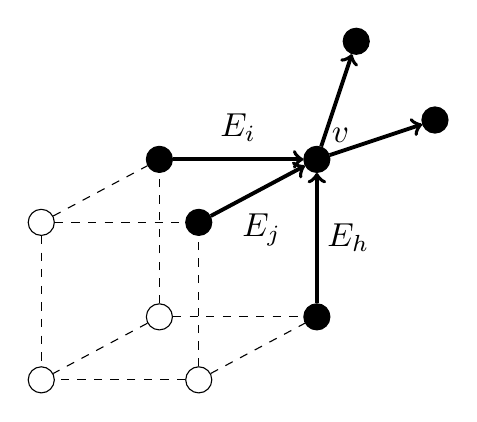
\begin{tikzpicture}

% NODES %%%%%%%%%%%%%%%%%%%%%%%%%%%%%%%%%%%%%%%%%%%%%%%%%%%%%%%%%%%%%%%%%%

\node[draw, circle, minimum height=0.2cm, minimum width=0.2cm, fill=black] (P0) at (6,6) {};

\node[draw, circle, minimum height=0.2cm, minimum width=0.2cm, fill=black] (P1) at (4,6) {};
\node[draw, circle, minimum height=0.2cm, minimum width=0.2cm, fill=black] (P2) at (4.5,5.2) {};
\node[draw, circle, minimum height=0.2cm, minimum width=0.2cm, fill=black] (P3) at (6,4) {};

\node[draw, circle, minimum height=0.2cm, minimum width=0.2cm, fill=black] (P1') at (6.5,7.5) {};
\node[draw, circle, minimum height=0.2cm, minimum width=0.2cm, fill=black] (P2') at (7.5,6.5) {};

\node[draw, circle, minimum height=0.2cm, minimum width=0.2cm] (P4) at (2.5,5.2) {};
\node[draw, circle, minimum height=0.2cm, minimum width=0.2cm] (P5) at (4.5,3.2) {};
\node[draw, circle, minimum height=0.2cm, minimum width=0.2cm] (P6) at (4,4) {};
\node[draw, circle, minimum height=0.2cm, minimum width=0.2cm] (P7) at (2.5,3.2) {};


% LINKS %%%%%%%%%%%%%%%%%%%%%%%%%%%%%%%%%%%%%%%%%%%%%%%%%%%%%%%%%%%%%%%%%%


\draw[->, line width = 1.4pt] (P1) -- (P0);
\draw[->, line width = 1.4pt] (P2) -- (P0);
\draw[->, line width = 1.4pt] (P3) -- (P0);

\draw[->, line width = 1.4pt] (P0) -- (P1');
\draw[->, line width = 1.4pt] (P0) -- (P2');

\draw[dashed] (P4) -- (P1);
\draw[dashed] (P4) -- (P2);
\draw[dashed] (P5) -- (P2);
\draw[dashed] (P5) -- (P3);
\draw[dashed] (P6) -- (P1);
\draw[dashed] (P6) -- (P3);
\draw[dashed] (P4) -- (P7);
\draw[dashed] (P5) -- (P7);
\draw[dashed] (P6) -- (P7);



% ETIQUETTES

\node[scale=1.2] at (5.0,6.4) {$E_i$};
\node[scale=1.2] at (5.3,5.1) {$E_j$};
\node[scale=1.2] at (6.4,5.0) {$E_h$};


\node[scale = 1.2] at (6.3,6.3) {$v$};

\end{tikzpicture}
